%First define the problem to be solved
\subsection{Problem Description}
As mentioned in Chapter \ref{chapter:introduction}, a major problem in hazardous scene management includes localizing sources of hazardous materials and localizing potential sources of evidence. The reasons these are difficult problems, in the context of the ROCSAFE project, are:
\begin{itemize}
    \item Hazardous materials may belong to different classes of threat, as outlined in the CBRN acronym. If the nature of the threat is uncertain, the wrong preventative measures may be taken and personnel may be put at risk. 
    \item Evidence localization usually requires moving a sensor to within close proximity of the evidence. If a human is responsible for this, there is a chance that they will accidentally tamper with the evidence, possibly yielding it unusable.
    \item Since these scenarios are highly dangerous, the area to search may be large to avoid potentially missing important sources of evidences. This means that the process of localization may be painstaking and time-consuming for humans.
\end{itemize}
This section proposes a system that can aid the execution of these tasks using a system of automated \textbf{U}nmanned \textbf{A}erial \textbf{V}ehicles (UAVs). \par



Spatiotemporal localization problems have a reasonable body of literature behind them, and can be described using abstract language which allows them to be approached using a common framework, with only minor implementation details necessary to specify which instance of the problem is being addressed. The framework we have developed uses a lot of the theory outlined in the Background Knowledge chapter and builds on existing literature. The problem that this chapter (section) attempts to solve can be generally described as follows: \par

\textit{Given a region of space to explore and a set of heterogeneous autonomous aerial vehicles with sensing capabilities, devise a search strategy which will return either the locations of the targets if one or more is present, otherwise return that no targets are present.} \par

Concrete versions of this that are later addressed are:
\begin{itemize}
    \item \textit{Given a system of heterogeneous autonomous aerial vehicles, some of which are equipped with radiation sensors and limited battery capacity, localize multiple sources of radioactive material in a scene.}
    \item \textit{Given a system of heterogeneous autonomous aerial vehicles, some of which are equipped with high-quality cameras and limited battery capacity, localize multiple objects of a given description in a scene.}
\end{itemize}
%not sure whether I should mentioned about battery etc. here or to let the discussion lead to this naturally.
\par

\note{Did not attempt to solve this full problem in one go, instead took a simplified version and then gradually added in constraints.}

\subsection{Initial Assumptions}
\note{may need to rename this. want to convey that initially, we made some simplifying assumptions that isolate key aspects of problem that need to be solved. Then these assumptions were modified to deal with the more complex problem involving battery etc.}

Rather than immediately attempting to tackle the full problem, we chose to initially make some simplifications in order to identify potential solution strategies that could be extended to more complex versions of the problem. At the outset, we made the following simplifying assumptions:
%As outlined in the literature review, this problem has been approached before by treating the problem as a 2 Time Slice Dynamic Bayesian Network (2TDBN). 
\begin{itemize}
    \item There are either zero or one targets to be localized.
    \item The UAVs have unlimited battery capacity.
    \item The region that the UAVs need to search can be well approximated by a polygon.
    \item The sensor specificity and sensitivity are known or can be estimated for a given resolution (e.g. 1m). These are assumed to be greater than 50\% for the given resolution.
    \item The UAVs operate over a discrete spatial grid spanning the region to search, assumed to be polygonal as above, the dimensions of which are pre-determined by the sensor resolution.
    \item The UAVs are assumed to have a GPS sensor that is accurate to beyond the sensor resolution (implying that the UAV moves to discrete grid locations without drift).
    \item The target is assumed to be small enough to occupy only one grid cell at a time. It is also assumed to not lie across grid cells.
\end{itemize}
While these assumptions are clearly unrealistic, they are convenient because they simplify the design of the system and subsequent analysis. In later sections in this chapter, these assumptions are relaxed and the necessary modifications for the solution strategy are discussed. Some ramifications of these assumptions are addressed later in the chapter, at section <x>. It is worth noting that similar simplifying assumptions were made in related works in the literature, 
(\cite{Chung2007ASearch} and \cite{Waharte2010SupportingUAVs}), % find additional citations in mendeley
which strongly influenced our initial approach.

%Outline experimental setup
\subsection{Experimental Testbed}
Given the assumptions outlined above, rather than beginning by working on designing candidate solutions, we instead decided to set up the software that would be necessary to quickly test and evaluate a solution. This is related to the specification of the agent's environment, which is described in subsection \ref{subsection:intial_agent_design}. This involved the following software components:
\begin{itemize}
    \item A 2-Dimensional grid coordinate system which can be easily configured to create a grid over a polygonal region. This is outlined in greater detail in section <provide a reference to the section>.
    \item An evidence source simulator which simulates the readings that a sensor would observe given the sensitivity and specificity of the sensor.
    \item A grid manager component, which manages the positions of UAVs and targets on the grid.
    \item A simulation manager component, which constructs the agents from their configuration files and is responsible for running the simulation using the other software components.
    \item Configuration files which allow the user to specify the configurations of the sensors, the agents, environment parameters and debugging/analysis files.
\end{itemize}
These components were designed in a modular fashion to distinguish the agent from its environment, shown in Figure \ref{fig:agent_env_interaction}. This seems like an obvious and intuitive practice, but can be easily overlooked while writing code. For example, the agent may have an internal representation of the grid environment in which it operates which should be completely independent of the actual grid environment which is run in the simulation. The user can fully specify all aspects of the agent and environment (relating to the above assumptions) through configuration files. \note{Maybe include an example figure showing a config file.}

%Discuss solutions explored - not sure how to address the modularity associated with this.
%\subsection{Identifying Components of the Problem}


\subsection{Prefatory Agent Design}\label{subsection:intial_agent_design}
\note{addressed some of these simultaneously (i.e. once I had decided model-based agent, then had to answer question of what model will look like)}
\note{probably best to list these individually with some corresponding discussion}

This section begins by describing four critical parts of the agent design, collectively referred to as the agent's \textit{task environment}: the Actuators, Sensors, Environment, and Performance Element. Further discussion on specific aspects of how the agent function was implemented is then given.
%where the larger multi-faceted problem is broken down into smaller individual sub-problems. 

\subsubsection{Agent Environment}
\note{Use of italics may not be necessary here}
\note{Should refer to previous works more here}
Here, we refer to conventional terms used to describe agent environments, described in \cite[p.~41]{AIAMA}. The agent's environment is \textit{partially observable}, since it is assumed that it cannot directly observe the location of the target, but must instead use partial information related to the location of the target from noisy sensors. The outcomes of the agent's actions are assumed to be \textit{deterministic}, meaning that if an agent chooses to move to a location, it is assumed to do so without any chance of it accidentally moving to an alternative location. The environment is \textit{sequential}, arising from the fact that future decisions on where the agent should take a sensor reading are influenced by previous locations at which a sensor reading has been taken. The agent is assumed to operate in a 2-dimensional environment, consisting of discrete uniformly spaced grid cells overlaid onto a physical region of space. The environment state can then defined by the tuples of the unknown location of the target with the search status. The unknown location of the target can be described by the set
\[\{x_1, x_2, ..., x_n, x_{n+1}\}\]
where $x_i$ represents the target location being at grid cell $i$ for $i \in \{1, 2, .., n\}$, and $x_{n+1}$ represents that the target is not present. The search status can be described by 
\[ \{ONGOING, TERMINATED\_x_1, TERMINATED\_x_2, ..., TERMINATED\_x_n, TERMINATED\_x_{n+1}\} \]
where $ONGOING$ represents that the search is continuing and $TERMINATED\_x_i$ is an absorbing terminal state that arises from the agent taking a terminal action indicating the target location, explained further in the subsequent paragraph. It is necessary to include the terminal states in the environment representation in order to specify \textit{goal states} and a \textit{performance measure} for the agent. The Cartesian product of these sets defines the environment state.
\note{Goal state not explicitly mentioned - might need to modify definitions to be able to include one.}

\subsubsection{Actuators and Sensors}
Here we consider the actions that may be chosen to be performed by actuators and percepts that may be received by sensors. The problem of \textit{target localization} in the context of this chapter requires the agent to move around a discrete grid and use a calibrated sensor to record noisy readings that indicate whether the target is present or not at the location of the reading. It is therefore intuitive to describe the set of possible actions to be performed by the actuators by the set of all $n$ possible grid locations that the agent can move to and take a sensor reading at, indexed by an arbitrary ordering: $\{location_1, location_2, ..., location_n\}$. We add additional actions to this set, $\{TERMINATE\_SEARCH\_x_{i}\}$, for $i \in \{1, 2, ..., n, n+1\}$, which lead to an absorbing terminal state representing the agent's conclusion regarding whether a target is present or not, $TERMINATE\_SEARCH\_x_{i}$ . The set of percepts that the agent will receive from its sensors come from the binary set \{1, 0\}, indicating the target has or has not been detected, respectively.



\subsubsection{Performance Measure}
The agent's performance measure maps sequences of environment states to the real numbers. Given the above definitions, it is clear that environment states of the form
\[ <x_i, TERMINATED\_x_i> \]
should be of high value (as they indicate that the agent has correctly identified the location of the target in the environment). Secondary to this, longer percept sequences should have a lower value than shorter percept sequences. Therefore, the performance measure primarily gives high values to the agent when it correctly identifies the location of the target or correctly concludes that the target is not present, with a secondary ordering on value determined by the time taken to come to a conclusion. This can be defined as:
\note{Be careful that this agrees with the rest}
\[
Performance Measure(state_1,..., state_t) = 
\begin{cases}
\frac{1}{t} \quad \text{ if } state_t \text{ = } <x_i, TERMINATED\_x_i>
%agent returns correct target location.} 
\\
-1 \quad \text { otherwise. }
\end{cases}
\]

%\[
%Performance Measure(state_1,..., state_t) = 
%\begin{cases}
%\frac{1}{t} \quad \text{ if } state_t \text{ = } <x_i, TERMINATED\_x_i>
%agent returns correct target location.} 
%\\
%\frac{1}{t} \quad \text{ if agent correctly returns target is not present.}
%\\
%-1 \quad \text { if agent returns incorrect target location.}
%\\
%-1 \quad \text{if agent incorrectly returns target is not present}
%\end{cases}
%\]

It is worth noting that this performance measure suggests goal states for the agent:
\[ <x_i, TERMINATED\_x_i> \]

\subsubsection{Agent Function Design}
Once key components of the agent and it's environment were identified, we began working on the design of the agent function. In Chapter \ref{Background}, four common classes of agents were identified, based on the design of their corresponding agent function. Using this list as a reference, we decided that a model-based agent would be a suitable starting point, since model-based agents can maintain internal state to handle problems associated with partial observability \cite{AIAMA}.

intuitively help guide the search process. On initial contemplation, a goal-based agent would seem to be a good fit , however there is an outstanding issue that cannot easily be addressed: defining a goal state cannot be done directly, since the agent's sensors are assumed to be noisy. This means that just because a positive reading is reported doesn't mean that the search can be terminated, due to that fact that the sensor reading could be spurious. Therefore, a model-based, utility-based agent is the obvious choice of agent design, since a utility function can help guide that agent towards a  without knowing the exact specification of the goal state. A good example of the architecture of a model-based, utility-based agent is shown in figure \ref{fig:model_based_utility_based}.
\begin{figure}
    \centering
    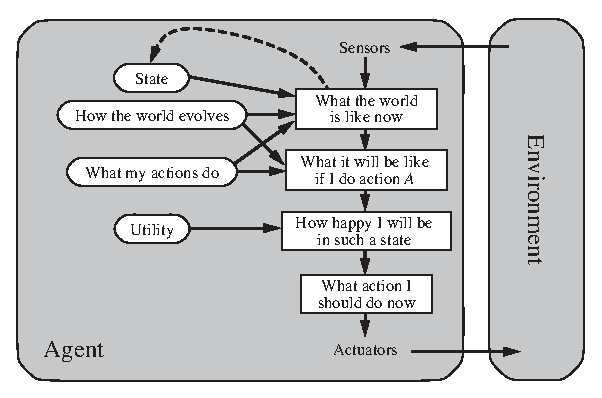
\includegraphics{Chapters/MultiAgentTargetDetection/BayesianFiltering/Figs/utility-based-agent.eps}
    \caption{Figure based on Model-Based, Utility-Based Agent Architecture (Russell and Norvig)\cite[p.~54]{AIAMA}}
    \label{fig:model_based_utility_based}
\end{figure}


\subsubsection{Stochastic World Model}
\placeholder



\subsubsection{Internal state}
\placeholder

\subsubsection{Action Selection Strategy}
\placeholder

\subsubsection{Search Cutoff Strategy}
\placeholder


\subsubsection{Implementing the Agent}
\placeholder

\subsubsection{Initial Results}
\placeholder

\subsection{Incorporating Battery Capacity Constraints}
\placeholder

\subsubsection{Incorporating Multiple Targets}
\placeholder

\subsubsection{Incorporating Multiple UAVs}
\placeholder



\begin{enumerate}
    \item How to design the agent function, as discussed in chapter \ref{Background}.
    \item What kind of model can be used to describe the agent's environment (assuming using a model-based, utility-based agent function design).
    \item What kind of internal state does the agent need to maintain.
    \item When should the agent cutoff its search for the target?
    \item How should the agents choose actions to perform based on its model of the environment?
    \item What percepts will the agent receive and what actions will it perform? How can these be represented using software?
\end{enumerate}

The target detection problem described in this thesis naturally decomposes into a number of sub-problems. %These components aren't independent, might be worth discussing how the components interact.

One component is obviously the world model, which is the agent's internal representation of the world and it's dynamics. The agent maintains an internal state
\subsubsection{Results}
%How to break this down - by control strategy, problem type etc.?

\subsection{Discussion and Conclusions}
\subsubsection{Limitations}
%Talk about  problem of grid resolution, drift may be an issue if GPS not present (this could be addressed by assuming that an initial mapping phase is carried out, so mapping is all that's necessary to keep track of location while searching)